\documentclass[a4paper,11pt]{article}
\usepackage{exptech}
\usepackage{textcomp}
\usepackage{graphicx}
\usepackage{array}
\usepackage[babel=true]{csquotes}
\usepackage{url}
\usepackage{hyperref}
\usepackage{wrapfig}
\usepackage[export]{adjustbox}
\usepackage{titletoc}

\titlecontents{subsection}[3.8em]{}{}{}{}[\addvspace{-0.5pt}]
\hypersetup{
  bookmarks=true, % show bookmarks bar?
  pdftitle={Avalon - Rapport de spécifications fonctionnelles}, % title
  pdfnewwindow=true, % links in new window
  colorlinks=true, % false: boxed links; true: colored links
  linkcolor=black, % color of internal links (change box color with linkbordercolor)
  citecolor=cyan, % color of links to bibliography
  filecolor=cyan, % color of file links
  urlcolor=cyan % color of external links
}

\title{
  \textbf{Avalon}\\
  Rapport de spécifications fonctionnelles
}
\markright{Avalon - Rapport de spécifications fonctionnelles}
\author{
\begin{minipage}{0.4\textwidth}
	\begin{flushleft} \large
		\emph{Auteurs :}\\
		Alexandre \textsc{Audinot}\\
		Julien \textsc{Bouvet}\\
		Cyrille \textsc{Delabre}\\
		Thierry \textsc{Gaugry}\\
		Nicolas \textsc{Hurman}\\
		Léo \textsc{Jacoboni}\\
		Alexandre \textsc{Leonardi}\\
	\end{flushleft}
\end{minipage}
\begin{minipage}{0.4\textwidth}
	\begin{flushright} \large
		\emph{Encadrants :} \\
		Valérie \textsc{Gouranton}\\
		Ronan \textsc{Gaugne}\\
		Bruno \textsc{Arnaldi}\\
		Willy \textsc{Allègre}\\
		Jean-Paul  \textsc{Departe}\\
	\end{flushright}
\end{minipage}
}

\date{23 Octobre 2014}

\begin{document}
\maketitle
\thispagestyle{empty}
\begin{abstract}
\textbf{Avalon :} Environnement de Réalité Virtuelle pour l'apprentissage à l'utilisation d'appartements tremplins. Réalisation en 3D d'un appartement domotisé interactif utilisé dans le cadre de la rééducation des personnes handicapées.
Le projet est proposé par le centre mutualiste de rééducation et de réadaptation fonctionnelles de Kerpape (plus particulièrement les ingénieurs du laboratoire électronique Willy Allègre et Jean-Paul Departe).
Le modèle 3D de l'appartement nous est fourni, et notre travail consistera à réaliser un logiciel fonctionnel permettant de se déplacer dans l'appartement et implémentant les interactions avec les différents éléments de domotiques, en plus de prendre en charge différents périphériques de contrôle. 
\end{abstract}

\begin{figure}[h!]
	\centering
	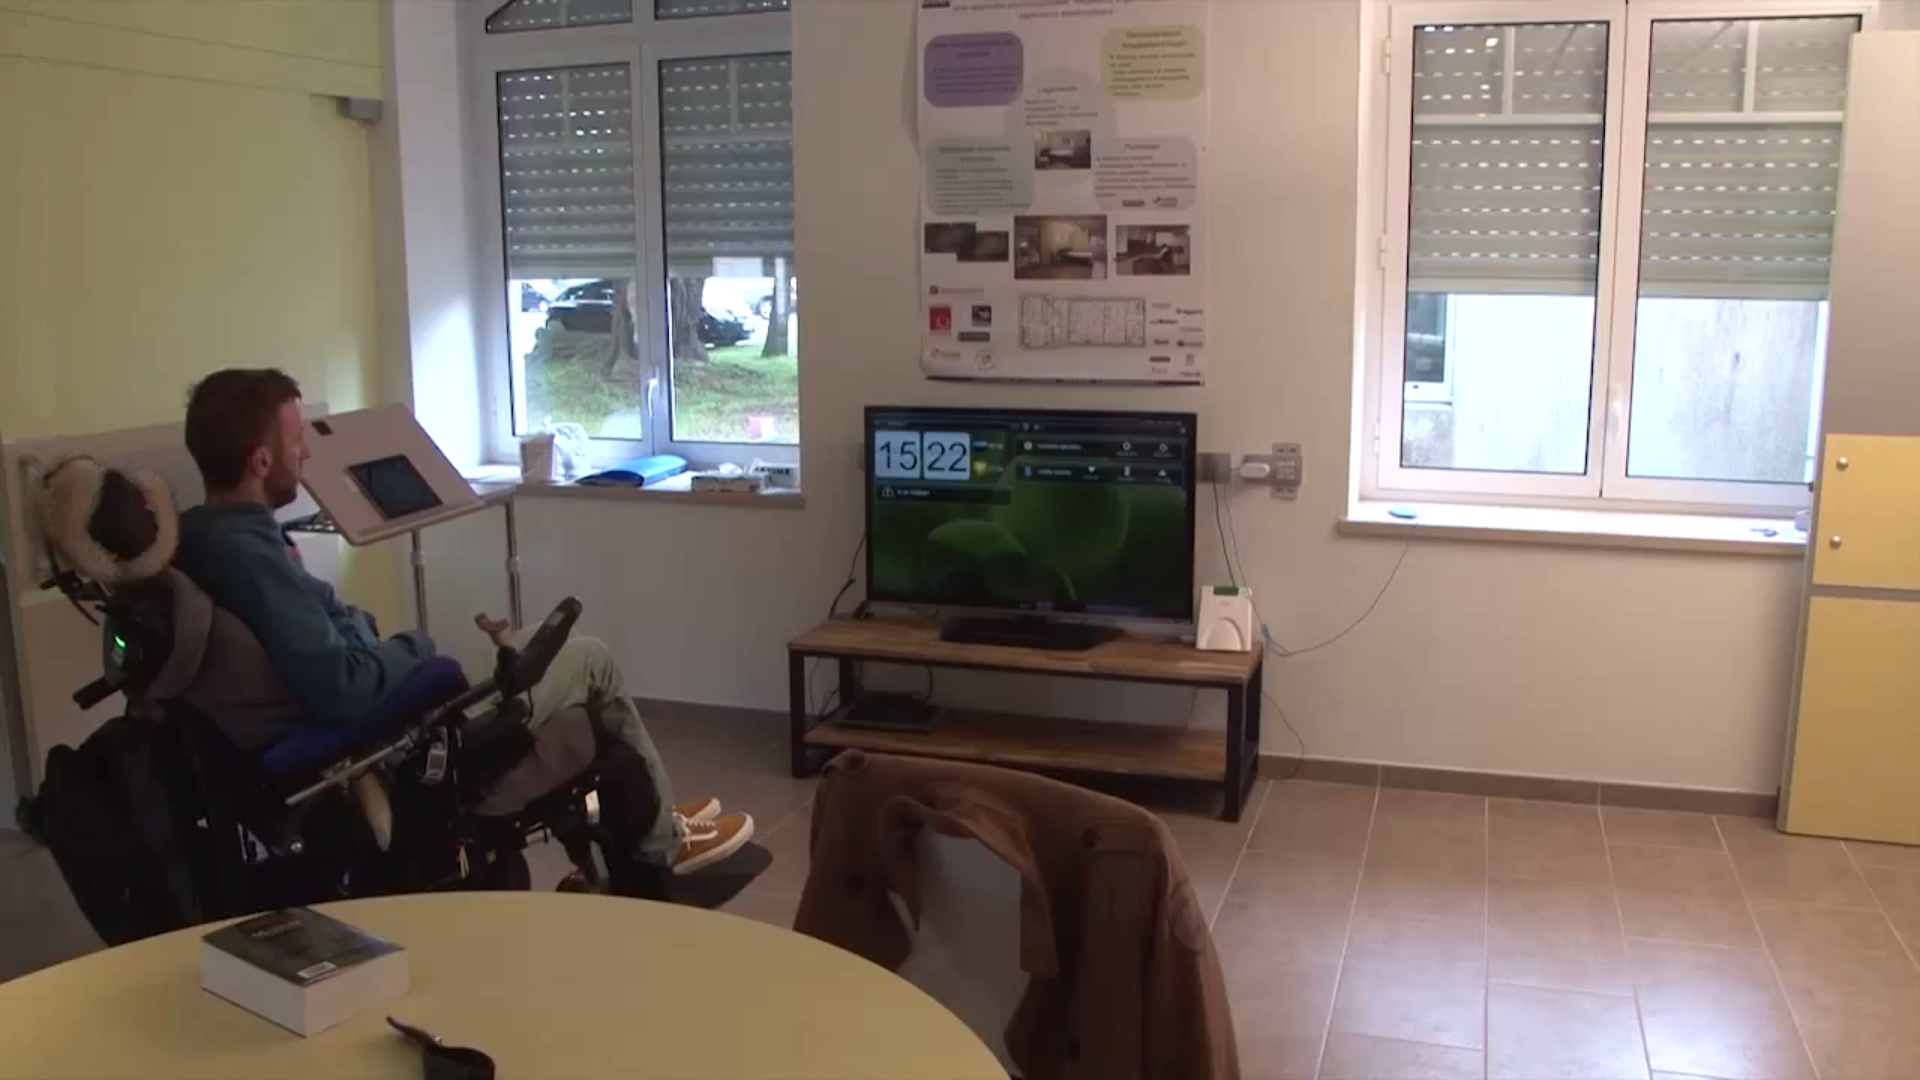
\includegraphics[height=170pt]{2-Specifications/img/screen_appart.png}
\end{figure}

%\vfill
%[width=\textwidth]
\begin{figure}[h!]
   \begin{minipage}{0.3\linewidth}
      
\includegraphics[scale=0.9]{2-Specifications/img/logo_insa.jpeg}
   \end{minipage} 
   \begin{minipage}{0.2\linewidth}
      \centering
      
\includegraphics[scale=0.5,left]{2-Specifications/img/logo_irisa.jpg}
   \end{minipage}\hfill
   \begin{minipage}{0.2\linewidth}
      
\includegraphics[scale=0.9]{2-Specifications/img/logo_kerpape.png}
   \end{minipage}
\end{figure}

\pagebreak

\tableofcontents
\pagebreak


\section{Introduction}

% Annonce plan
% Visite kerpape
% Rencontre clients
\begin{wrapfigure}{r}{0mm}
	\centering
	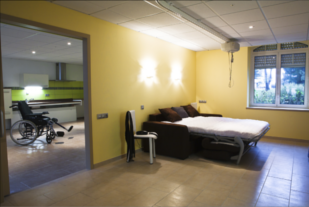
\includegraphics[scale=1]{1-PreEtude/img/appt_tremplin_intro.png}
\end{wrapfigure}
Notre projet consiste en la modélisation d'appartements tremplins en 3D pleinement interactifs, dans lesquels des personnes handicapées pourront évoluer et apprendre à se servir des différents équipements de domotique présents. 
Le projet est proposé par le centre de rééducation de Kerpape et par l'IRISA, ce qui lui confère un intérêt particulier à nos yeux car le commanditaire est extérieur à l'école, et le projet répond donc au besoin d'un véritable client de la même manière que le ferait un projet rencontré dans notre vie professionnelle. 
Ainsi, nous avons eu l'occasion de nous entretenir avec Willy Allègre et Jean-Paul Departe, ingénieurs de Kerpape à l'origine du projet, tout d'abord lors d'une conférence téléphonique pendant laquelle ils nous ont décrit ce qu'ils attendaient de l'application. Par la suite, un déplacement au centre de Kerpape nous a permis de parfaire l'image que nous nous faisons du résultat attendu et de compléter le cahier des charges de la future application. \newline

\begin{wrapfigure}{l}{0mm}
	%\cite{archeologie}
	\centering
	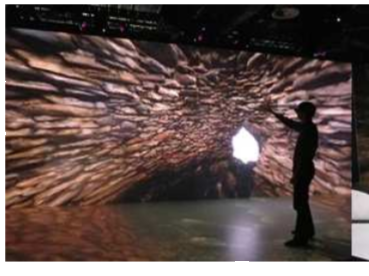
\includegraphics[scale=0.5]{1-PreEtude/img/rv_2.png}
\end{wrapfigure}
Au cours de cette étude de pré-spécifications, nous commencerons par définir plus précisément le contexte de notre projet, en tentant de cerner ce qu'est la réalité virtuelle et son importance dans le domaine de la santé. 
Nous présenterons ensuite le cahier des charges en deux parties, d'abord d'un point de vue fonctionnel, les différentes fonctions qui sont attendues de notre applications, et ensuite d'un point de vue technique, les différentes contraintes que nous aurons à respecter. 
Après cela nous décrirons, dans l'étude fonctionnelle, les différents scénarios types qui nous ont été proposés par Kerpape et auxquels les patients devront pouvoir être confrontés. 
Puis nous spécifierons les différents logiciels à notre disposition ainsi que les différents matériels, et les périphériques que nous prévoyons de rendre utilisables. 
Enfin, nous ébaucherons une planification prévisionnelle du travail à fournir tout au long de l'année. 
\pagebreak
\section{Spécifications fonctionnelles du projet}

Dans notre rapport précédent, nous définission un cahier des charges qui s'articulait principalement autour de 3 grands axes qui étaient les suivants :
\begin{itemize}\renewcommand{\labelitemi}{$\bullet$}
\item Présence d'interactions avec l'environnement
\item Applications aisément portable vers différents systèmes d'utilisation
\item Exploitation de différents périphériques d'entrée/sortie
\end{itemize}
Nous allons donc dans un premier temps présenter les solutions techniques que nous avons retenues pour la réalisation du projet, en détaillant de quelle façon elles répondent à ces 3 problématiques, pour ensuite présenter un diagramme de cas d'utilisation qui résumera le fonctionnement global de l'application.

\subsection{Solutions techniques retenues}
La réalisation de notre projet s'appuiera donc principalement sur trois environnements de travail, Unity3D, Blender et MiddleVR.

\subsubsection{Unity : le moteur de rendu 3D}
L'utilisation d'Unity était imposée, en vertu des nombreux avantages du logiciel. Unity est un moteur de rendu 3D
\begin{wrapfigure}{l}{0mm}
	\centering
	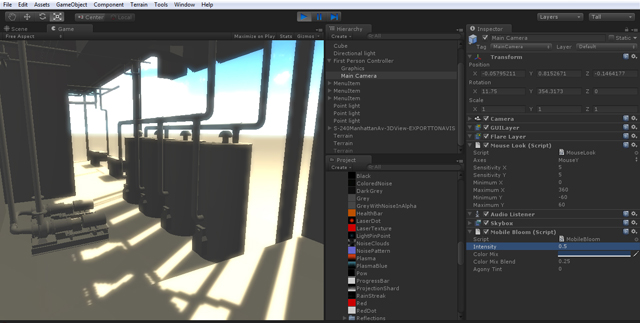
\includegraphics[scale=0.5]{2-Specifications/img-utilisateur/screen_unity.jpg}
\end{wrapfigure}
utilisé principalement pour la réalisation de jeux vidéos, et qui dispose d'une version gratuite. Très complet, il propose les différentes fonctionnalités dont nous avons besoin : il permet d'ouvrir le modèle 3D de l'appartement tremplin qui nous a été fourni par le centre de Kerpape, et de le modifier. \newline

Il permet aussi de réaliser les interactions entre utilisateur et environnement qui nous intéressent, que ce soit l'appui sur les différents interrupteurs gérant l'éclairage et l'ouverture/fermeture des volets, ou bien l'utilisation de la télécommande dont disposent les résidents de l'appartement qui centralise la plupart des actions qu'ils peuvent effectuer.
Enfin dernier avantage de Unity, il propose différentes cibles de compilation. En effet, même si dans un premier temps nous allons développer une application qui fonctionnera sous Windows 7 ou 8 avec un ensemble clavier/souris, nous aimerions ne pas être limités à cet environnement par la suite. \newline

Néanmoins, un problème est survenu lors de l'utilisation de Unity : le modèle 3D de l'appartement qui nous avait été fourni avait été créé grâce à 3DSMax, et les deux logiciels sont réputés incompatibles entre eux, ce qui s'est avéré dans notre cas. Nous avons donc au final obtenu un modèle contenant les volumes, mais sans texture ni lumière, que nous avons dû ajouter nous-mêmes.

\subsubsection{Blender : le logiciel de modélisation}
Blender est le logiciel de modélisation que nous allons utiliser pour les modifications du modèle qui nous a été fourni. Contrairement à Unity, il ne nous a pas été imposé, mais s'est dégagé comme étant le choix idéal du fait de la documentation imposante disponible sur le net et de sa gratuité.\newline

La majorité de l'appartement tremplin a déjà été modélisé pour nous, mais il reste néanmoins quelques détails à rajouter, comme l'interphone/téléphone (le domophone), ou encore le panneau d'interrupteurs à l'entrée de l'appartement. Nous nous en servirons de plus pour corriger les pertes rencontrées lors de l'import du modèle 3D sous Unity : rajouter la lumière et les textures à notre modèle.

\subsubsection{MiddleVR : la gestion des périphériques d'interaction}

MiddleVR répond au troisième des objectifs que nous nous sommes fixés : exploiter différents périphériques d'entrée/sortie. En effet, pour ce faire, il fallait pouvoir s'abstraire desdits périphériques au cours du développement de l'application. L'idée est de développer toutes les fonctionnalités qui nous intéressent, l'utilisation des différents interrupteurs, etc, et d'ensuite disposer d'un moyen facile d'associer l'usage d'un périphérique donné à une fonctionnalité donnée.\newline

Or c'est précisément ce que nous permet MiddleVR. Prenant la forme d'un plugin Unity disponible gratuitement, il est capable de reconnaître les différents périphériques de réalité virtuelle à notre disposition, pour ensuite les associer à certaines actions.

\subsection{Scénarios d'utilisation}
Le cahier des charges qui nous a été fourni par le centre de Kerpape prévoit l'implémentation de différents scénarios d'utilisation centrés sur l'usage du domophone et que nous avons détaillés dans le premier rapport :
\begin{itemize}\renewcommand{\labelitemi}{$\bullet$}
\item Appel téléphonique normal
\item Appel \textit{via} l'interphone d'une personne venant fréquemment (un infirmier par exemple)
\item Appel \textit{via} l'interphone concernant une visite inattendue
\end{itemize}
Ces scénarios mettent en avant l'usage particulier qui peut être fait du téléphone et de la télévision (cf. \textsc{figure~\ref{domophone}}), car ceux-ci servent d'interphone, respectivement pour le son et l'image. Il faut donc que le téléphone, dans notre application, puisse recevoir des appels des deux types différents, mais aussi que la TV puisse recevoir le flux vidéo de l'interphone (en pratique dans les appartements tremplins, l'habitant doit se placer sur le canal 80 pour afficher la caméra de l'interphone).
\begin{figure}[h!]
	\begin{center}
  		\caption{Cas d'utilisation du domophone}
  		\label{domophone}
  		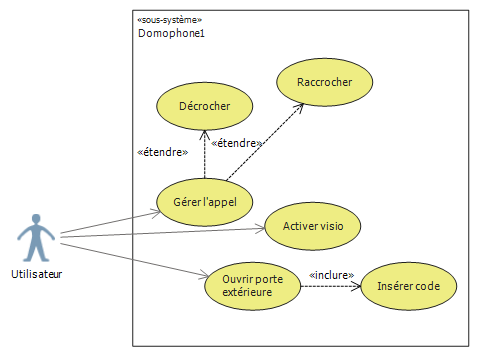
\includegraphics[width=\textwidth]{2-Specifications/img-utilisateur/use_case_diag.PNG}
  	\end{center}
\end{figure}

\subsection{Déploiement}
Parmi nos 3 axes de développement, l'un était l'exploitation de différents périphériques d'entrée/sortie. Il y a, en pratique, 3 périphériques de sortie que nous prévoyons d'utiliser au cours du projet : un écran de PC classique, un casque de réalité virtuel type Occulus Rift, et la salle immersive Immersia de l'IRISA.

\subsubsection{Ecran}
Il s'agit de la première version que nous allons développer. Cette version pourra reconnaître différents périphériques d'entrée, mais sera au départ prévue pour des interactions via le couple clavier/souris. Grâce à MiddleVR, cette option n'est pas plus ou moins facile à implémenter que les autres, mais elle représente un bon point de départ car elle ne nécessite pas d'équipement particulier, le centre de Kerpape disposant déjà de machines qui pourront faire tourner le programme. \newline

De  plus, bien que cette approche soit moins \enquote{naturelle} que l'usage de dispositifs de réalité virtuelle comme ceux associés à la salle Immersia, elle est au final aisée de prise en main car il s'agit de matériel auquel la plupart des gens sont déjà habitués.

\subsubsection{Casque de RV}
La première approche présentée, bien qu'étant la plus pratique, n'implique pas suffisament la notion de réalité virtuelle qui est au coeur de notre projet. De plus, un dispositif comme un casque de réalité virtuelle permet une immersion plus totale de l'utilisateur.

Qui plus est, elle se marie avantageusement avec l'usage de dispositifs comme des manettes pour Nintendo Wii ou des Razer Hydra qui sont eux-mêmes plus immersifs que le classique clavier/souris, car ils permettent de retranscrire les mouvements réels que l'utilisateur fera avec ses mains. \newline
\begin{wrapfigure}{r}{0mm}
  \centering
  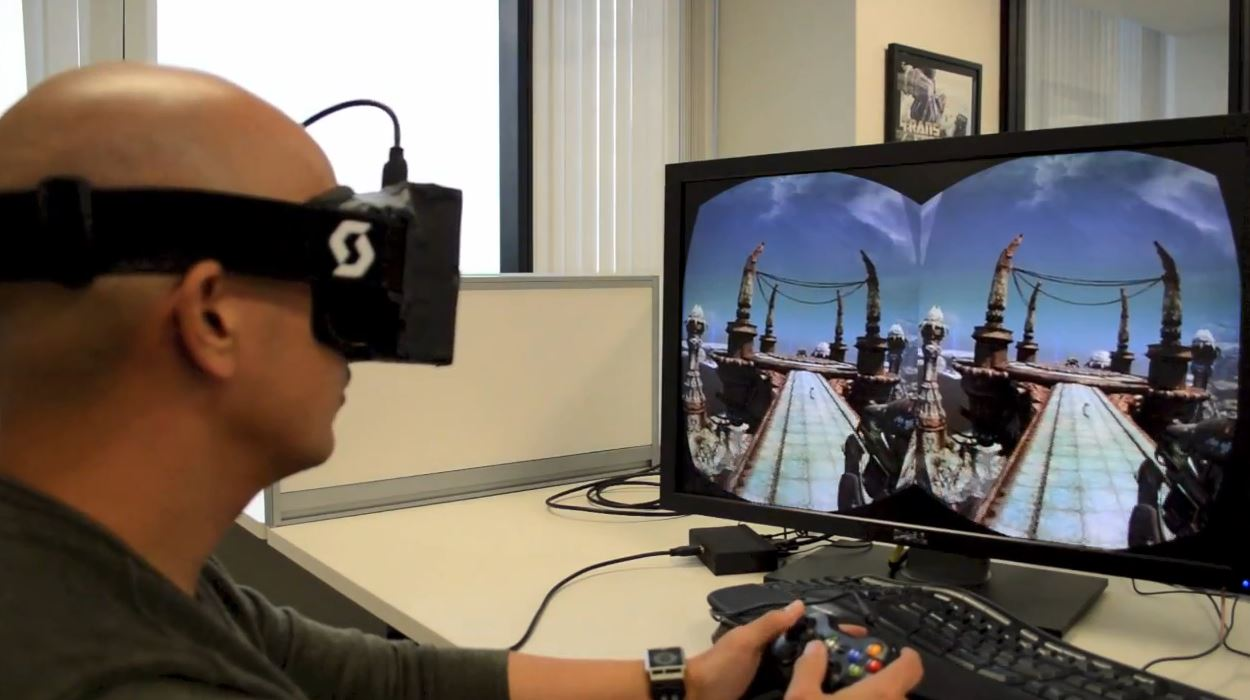
\includegraphics[scale=0.3]{2-Specifications/img-utilisateur/occulus.jpg}
\end{wrapfigure}
Lors de notre visite au centre de Kerpape nous avons fait essayer une démonstration de l'Occulus Rift à Willy Allègre et Jean-Paul Departe, qui ont été plutôt convaincus de l'intérêt du dispositif. Néanmoins, il s'agit d'une technologie onéreuse et dont le centre ne dispose pas actuellement.

\subsubsection{Salle immersive}
La salle immersive représente l'équipement de RV le plus complet dont nous puissions profiter et est donc une perspective de plate-forme très intéressante pour notre application.
\begin{wrapfigure}{l}{0mm}
	\centering
	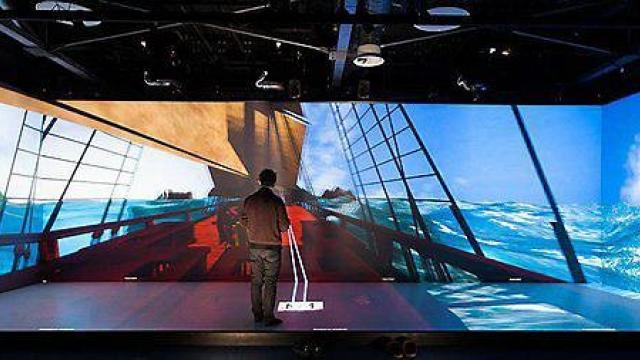
\includegraphics[scale=0.5]{2-Specifications/img-utilisateur/immersia.jpg}
\end{wrapfigure}
C'est l'option qui nous permettra les interactions les plus naturelles, car l'utilisateur se trouvera dans une projection à l'échelle 1:1 de l'appartement, équipé de lunettes 3D et de capteurs qui permettent de suivre la position des mains de l'utilisateur. \newline

Bien que Kerpape n'en dipose pas et n'ait pas la possibilité d'en utiliser une, l'implémentation du projet Avalon dans une salle immersive reste donc un objectif que nous souhaitons réaliser.

\pagebreak
\section{Spécifications niveau utilisateur}

Le logiciel destiné au milieu médical, doit tout d'abord être en mesure de répondre à une interface simple et compréhensible par tous les utilisateurs. Dans notre cas, l'utilisateur peut être le thérapeute ou le patient. L'objectif étant d'optimiser au mieux l'interaction entre les différents objets et l'utilisateur \textit{via} des périphériques accessibles et ergonomiques. Par ailleurs, il faut aussi considérer que le thérapeute doit pouvoir accéder aux différentes options et le modifier afin de faciliter l'utilisation et l'intéraction dans la scène pour le patient.
\newline
Nous verrons dans une première partie les différents modes de navigation possibles, puis comment l'utilisateur peut selectionner et déplacer les objets présents dans la scène en fonction du mode d'apprentissage, et enfin toute la partie de gestion des options du logiciel pour le thérapeute.


\subsection{Scénarios d'utilisation}
Le cahier des charges qui nous a été fourni par le centre de Kerpape prévoit l'implémentation de différents scénarios d'utilisation centrés sur l'usage du domophone et que nous avons détaillés dans le premier rapport :
\begin{itemize}\renewcommand{\labelitemi}{$\bullet$}
\item Appel téléphonique normal
\item Appel \textit{via} l'interphone d'une personne venant fréquemment (un infirmier par exemple)
\item Appel \textit{via} l'interphone concernant une visite inattendue
\end{itemize}
Ces scénarios mettent en avant l'usage particulier qui peut être fait du téléphone et de la télévision (cf. \textsc{figure~\ref{domophone}}), car ceux-ci servent d'interphone, respectivement pour le son et l'image. Il faut donc que le téléphone, dans notre application, puisse recevoir des appels des deux types différents, mais aussi que la TV puisse recevoir le flux vidéo de l'interphone (en pratique dans les appartements tremplins, l'habitant doit se placer sur le canal 80 pour afficher la caméra de l'interphone).
\begin{figure}[h!]
	\begin{center}
  		\caption{Cas d'utilisation du domophone}
  		\label{domophone}
  		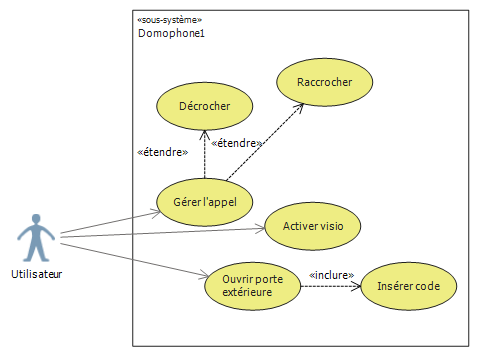
\includegraphics[width=\textwidth]{2-Specifications/img-utilisateur/use_case_diag.PNG}
  	\end{center}
\end{figure}

\subsection{Navigation}
Nous avons envisagé différents types de navigation au sein de l’environnement 3D, qui amèneront l’utilisateur à s’immerger et à interagir différemment avec la scène en fonction des périphériques utilisés.

\subsubsection{Exocentrée}
Avec un type de vue exocentré, l’utilisateur contrôle un avatar à la 3\up{ème} personne ce qui ne l’immergera pas totalement dans la scène. Cependant ceci peut permettre d'avoir une meilleure visualisation de la scène et de l'espace en 3D.
\newline
\textbf{Interface Souris - Clavier : }
L’utilisateur déplace son personnage à l’aide des touches du clavier. Il peut orienter la caméra l’aide de la souris. Pour entrer en interaction avec un objet il lui suffit de pointer l’objet avec la caméra et d’utiliser le clic gauche de la souris. L'orsqu'un objet est pointé il se met en légère sur-brillance. 
Dans cette interface on définit les boutons suivants :
	\begin{itemize}\renewcommand{\labelitemi}{$\bullet$}
  				\item bouton d’action : clic gauche de la souris
				 \item bouton de retour : touche \em{escape} du clavier
  				\item  bouton 2\up{ème} action : clic droit de la souris
			\end{itemize}
Le thérapeute pourra modifier ces réglages s'il souhaite faire interagir l'utilisateur avec des boutons différents.
\newline


\textbf{Interface WiiMote - Nunchuk : }
Pour déplacer l’avatar, l’utilisateur s'appuiera sur le joystick du Nunchuk. Il peut orienter la caméra l’aide de la Wiimote. Pour entrer en interaction avec un objet il lui suffit de pointer l’objet avec la caméra et d’utiliser un des boutons de la Wiimote :
	\begin{itemize}\renewcommand{\labelitemi}{$\bullet$}
  				\item bouton d’action : bouton A de la WiiMote
				 \item bouton de retour :bouton Z du Nunchuk
  				\item  bouton 2\up{ème} action : bouton B de la WiiMote
			\end{itemize}

\subsubsection{Endocentrée}
En point de vue endocentré, l’utilisateur est plongé totalement dans l’environnement. 
\newline
\textbf{Occulus Rift avec clavier-souis ou WiiMote-Nunchuk : }
De la même façon qu’en exocentré, l’utilisateur se déplacera et interagira avec la scène en utilisant l’interface clavier-souris ou WiiMote-Nunchuk. Cependant, on profite de ce point de vue immersif pour tirer profit des fonctionnalités de l’Occulus Rift.
Ce périphérique permettra la gestion de la caméra en orientant le champs de vision de l’utilisateur en fonction de ses mouvements de tête.
\newline
\textbf{Salle Immersia : }
La salle Immersia est une salle d’environnment 3D qui permet à l’utilisateur de s’intégrer totalement dans l’environnement virtuel. Ici une fois muni du capteur 3D dans l'espace, il pourra se déplacer totalement dans l’environnement.
Pour leur part les interactions seront effectuées grâce à une WiiMote.

\subsection{Sélection}

L'utilisateur, indépendamment du mode dans lequel il se trouve (Scénario ou déplacement libre), peut interagir avec son environnement pour effectuer certaines actions ou tâches demandées par le thérapeute. Il peut donc actionner certains objet et voir les actions qu'il a effectuées dans son environnement. Cependant ces actions sont dépendantes du mode d'apprentissage dans lequel il se trouve. En effet, trois modes sont disponibles : Symbolique, Assisté et Autonome. Nous verrons dans cette partie les différentes actions qui se produise en fonction du mode d'apprentissage lorsque l'utilisateur interagit avec son milieux. 

\subsubsection{Objets sélectionnables}

Avant de détailler le fonctionnement des différents modes, il est nécessaire d'expliciter les différents objets sélectionnables que l'on peut trouver dans l'appartement. On dénote dans la scène plusieurs objets qui permettent d'interagir avec le milieu :
\begin{itemize}
	\item Les interrupteurs pour les lumières, les portes internes et externes et les volets
	\item La télécommande qui comporte plusieurs boutons pour gérer notamment la télévision
	\item L'interphone qui permet de recevoir un appel
\end{itemize}

De même que précédemment, lorsque l'utilisateur pointe sur un objet, celui-ci se met en légère sur-brillance, il doit par la suite cliquer dessus pour pouvoir interagir avec. %Les interrupteurs, par un clic gauche (de la souris pas exemple), actionnent les différents éléments dans la pièce. %Pour la télécommande et l'interphone, le fonctionnement est un peu plus complexe : le premier clic permet d'avoir une vue zoomée sur l'objet et ainsi l'utilisateur peut selectionner le bouton qu'il souhaite actionner.


\subsubsection{Mode d'apprentissage : Symbolique}

La figure \ref{fig:MaquetteSymbolique} explique le fonctionnement lorsque l'utilisateur interagit avec un objet dans le mode symbolique. Elle est accompagné d'un diagramme d'activité (figure \ref{fig:CasUsageSymbolique}) pour une meilleur compréhension.
\newline
Lorsque l'utilisateur est dans un scénario ou dans un didacticiel, l'objet se met en sur-brillance dans la scène. L'utilisateur se déplace jusqu'à l'objet et rentre dans dans une vue symbolique qui lui explique le fonctionnement de l'objet. Dans notre exemple ici, pour l'ouverture d'une porte, l'utilisateur reçoit les consignes pour ouvrir la porte. Par exemple : « Le bouton du haut permet de fermer la porte, celui du bas de l'ouvrir. Si vous souhaitez ouvrir la porte il faut donc appuyer sur le bouton du bas ». Les consignes sont liées à des indications fléchées qui aident à la compréhension. Par la suite, l'utilisateur peut actionner le bouton. Cette action lance une animation qui montre de manière symbolique l'ouverture de la porte. 
\newline
En fonction du didacticiel plusieurs apprentissages peuvent se produire à la suite, ouverture de la porte puis fermeture par exemple. Si l'utilisateur ne souhaite plus interagir avec l'objet il peut a tout moment quitter la vue symbolique avec la touche «esc». 

\begin{figure}[h]
\centering
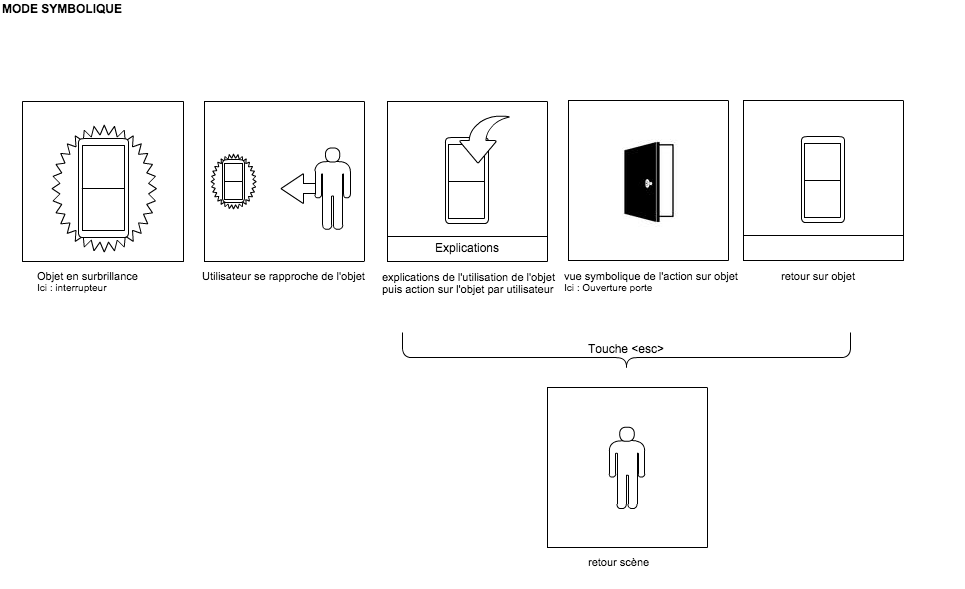
\includegraphics[width=1\textwidth]{2-Specifications/img-utilisateur/symbolique.png}
\caption{\label{fig:MaquetteSymbolique} Manipulation d'objets dans le mode Symbolique }
\end{figure}
\begin{figure}[h]
\centering
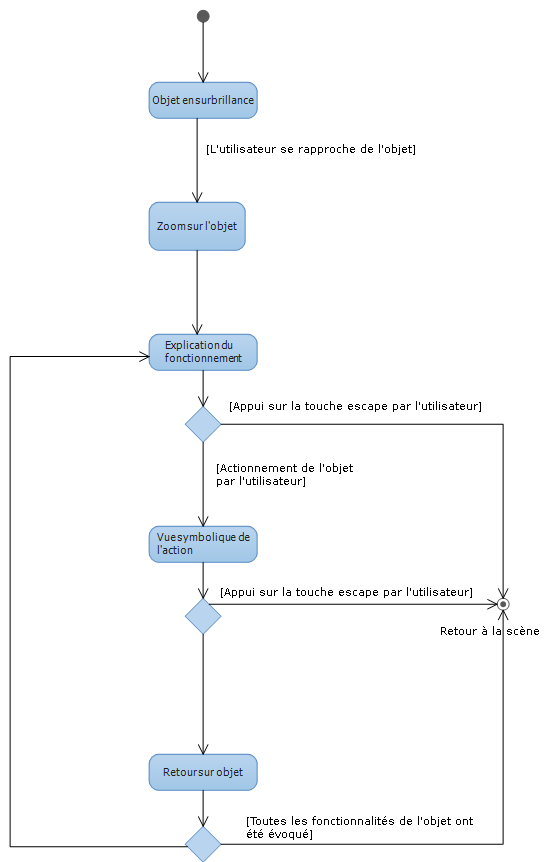
\includegraphics[width=1\textwidth]{2-Specifications/img-utilisateur/activite-symbolique.png}
\caption{\label{fig:CasUsageSymbolique} Diagramme d'activité : Manipulation d'objets dans le mode Symbolique }
\end{figure}
\FloatBarrier 


\subsubsection{Mode d'apprentissage : Assisté}

Après un apprentissage Symbolique, l'ergothérapeute peut décider de passer à un apprentissage Assisté. Dans ce dernier, l'utilisateur doit entreprendre plus d'actions que précédemment pour interagir avec l'objet. Comme précédemment, si l'utilisateur est dans un scénario ou didacticiel, l'objet se met en sur-brillance. L'utilisateur se rapproche alors et doit cliquer sur l'objet. Si celui-ci comporte plusieurs boutons (télécommande par exemple), une vue «zoomée» de l'objet apparaît et l'utilisateur peut cliquer sur le bouton qu'il doit actionner. Une fois le bouton cliqué, une fenêtre apparaît et montre en 3d l'action qui a été effectué. 
\newline
Les figures \ref{fig:MaquetteAssiste} et \ref{fig:CasUsageAssiste} reprennent le fonctionnement de ce mode.

\begin{figure}[h]
\centering
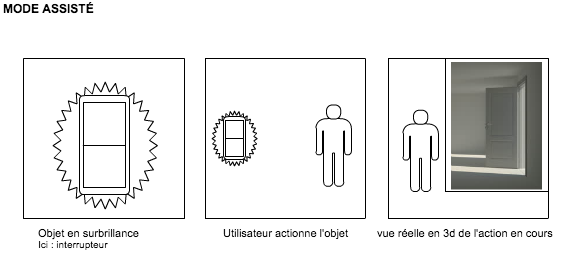
\includegraphics[width=1\textwidth]{2-Specifications/img-utilisateur/assiste.png}
\caption{\label{fig:MaquetteAssiste} Manipulation d'objets dans le mode Assisté }
\end{figure}
\begin{figure}[h]
\centering
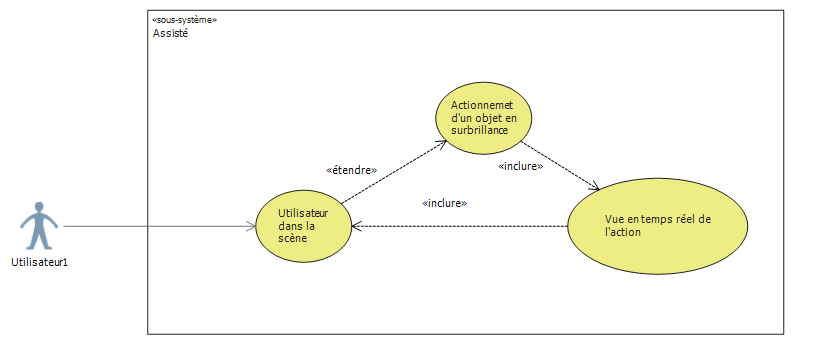
\includegraphics[width=1\textwidth]{2-Specifications/img-utilisateur/cas-usage-assiste.png}
\caption{\label{fig:CasUsageAssiste} Diagramme de cas d'usage : Manipulation d'objets dans le mode Assisté }
\end{figure}
\FloatBarrier 


\subsubsection{Mode d'apprentissage : Autonome}

Le mode autonome ne donne plus aucune indication à l'utilisateur. L'objet n'est plus en sur-brillance dans le cas de scénarios ou didacticiels. Il doit aller actionner lui même l'objet comme précédemment et se rendre compte en se déplaçant dans la scène si son action est bien la bonne. 
\newline
Les figures \ref{fig:MaquetteAutonome} et \ref{fig:CasUsageAutonome} reprennent le fonctionnement de ce mode.

\begin{figure}[h]
\centering
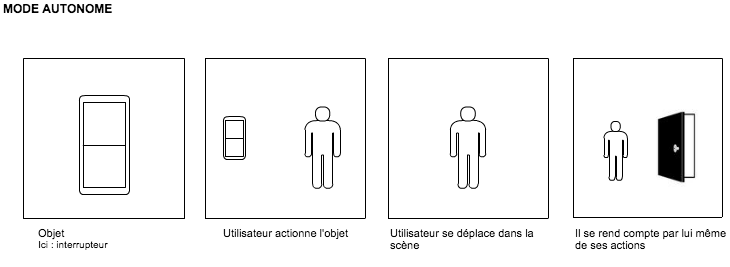
\includegraphics[width=1\textwidth]{2-Specifications/img-utilisateur/autonome.png}
\caption{\label{fig:MaquetteAutonome} Manipulation d'objets dans le mode Autonome }
\end{figure}
\begin{figure}[h]
\centering
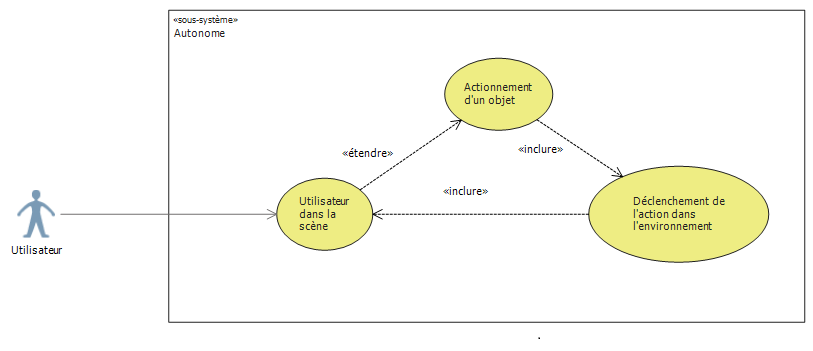
\includegraphics[width=1\textwidth]{2-Specifications/img-utilisateur/cas-usage-autonome.png}
\caption{\label{fig:CasUsageAutonome} Diagramme de cas d'usage : Manipulation d'objets dans le mode Autonome }
\end{figure}
\FloatBarrier 



\subsection{Manipulation}
Dans l’appartement, l’utilisateur est amener à manipuler différents types d’objet : un interphone, des interrupteurs et une télécommande

\subsubsection{Manipulation de l’interphone }
Une fois l’interphone sélectionné par l’utilisateur (par l’appui sur une touche ou automatiquement en fonction du mode d’apprentissage), ce dernier aura un affichage de l’appareil. Il pourra ensuite l’utiliser en appuyant sur ses touches grâce au pointeur de la souris ou de la Wiimote, (qui ne gère plus la caméra lors de ce type d’événement) et l’appui sur la touche d’action. La manipulation de l’interphone se termine lorsque l’utilisateur appuie sur la touche de retour ou qu’il a correctement terminé l’action à effectuer du scénario. L’utilisateur bascule alors sur l’appartement.

\subsubsection{Manipulation d’un interrupteur}
L’utilisateur s’approche de l’interrupteur, et l’actionne grâce à l’appui sur le bouton d’action. En fonction du mode d’apprentissage, il y a affichage centré ou non sur l’objet. Le retour à la scène se fait automatiquement une fois l’action terminé ou par l’appui sur la touche de retour.

\subsubsection{Manipulation de la télécommande}
Si l’utilisateur n’a pas encore pris la télécommande il peut aller la chercher dans l’environnement. Une fois qu’elle est sélectionnée, il peut l’utiliser grâce au pointeur de la souris ou de la WiiMote et à l’appui sur le bouton d’action. A tout moment, il peut la reposer grâce au bouton de retour. Ses actions terminées, il peut la reposer ou la garder avec lui en appuyant sur le bouton de deuxième action. 

\subsection{Contrôle d’application}
\subsubsection{Administrateur}
Pour le contrôle de l'application, le thérapeute sera considéré comme administrateur de l'application. Il a accès à 
tous les paramètres de configurations et choisir les différents modes (scénarios,didacticiels,balade libre) pour l'Utilisateur.
\newline
Les figures \ref{fig:Menu} et \ref{fig:CasUsageMenu} reprennent le fonctionnement global de l'interface. Ainsi sur le menu principal, le thérapeute peut choisir entre les Didacticiels, les Scénarios, se balader librement ou les Options.
\newline
Les Options permettent de configurer le choix des touches ainsi que certains paramètres plus personnalisés pour l'utilisateur. On peut ainsi charger/sauvegarder un fichier utilisateur avec les configurations des touches, taille de personnage, télécommande personnalisée, qui ont été au préalable déjà configurés. 

On peut aussi choisir, si la configuration le permet (Clavier/Souris, Occulus, Salle Immersia), le mode de Navigation (endocendré ou exocentré). 
\newline
Lorsque les configurations de bases ont été effectuées, le thérapeute peut alors choisir un des différents modes. Si l'on choisit un Scénario ou un Didacticiel, le mode d'apprentissage (Symbolique, Assisté, Autonome) sera demandé. Dans le cas de la balade libre, le mode d'apprentissage est Autonome par défaut. Le mode d'apprentissage peut-être ultérieurement changé dans le menu d'option de la scène si le thérapeute le souhaite. 
\newline

\begin{figure}[h]
\centering
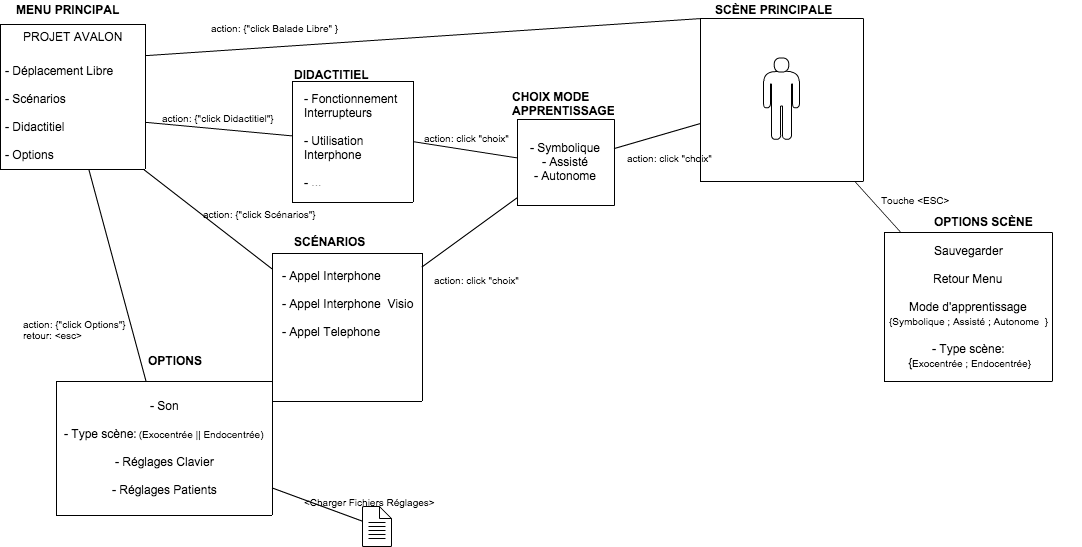
\includegraphics[width=1\textwidth]{2-Specifications/img-utilisateur/menu.png}
\caption{\label{fig:Menu} Menu principal et configurations environnement }
\end{figure}
\begin{figure}[h]
\centering
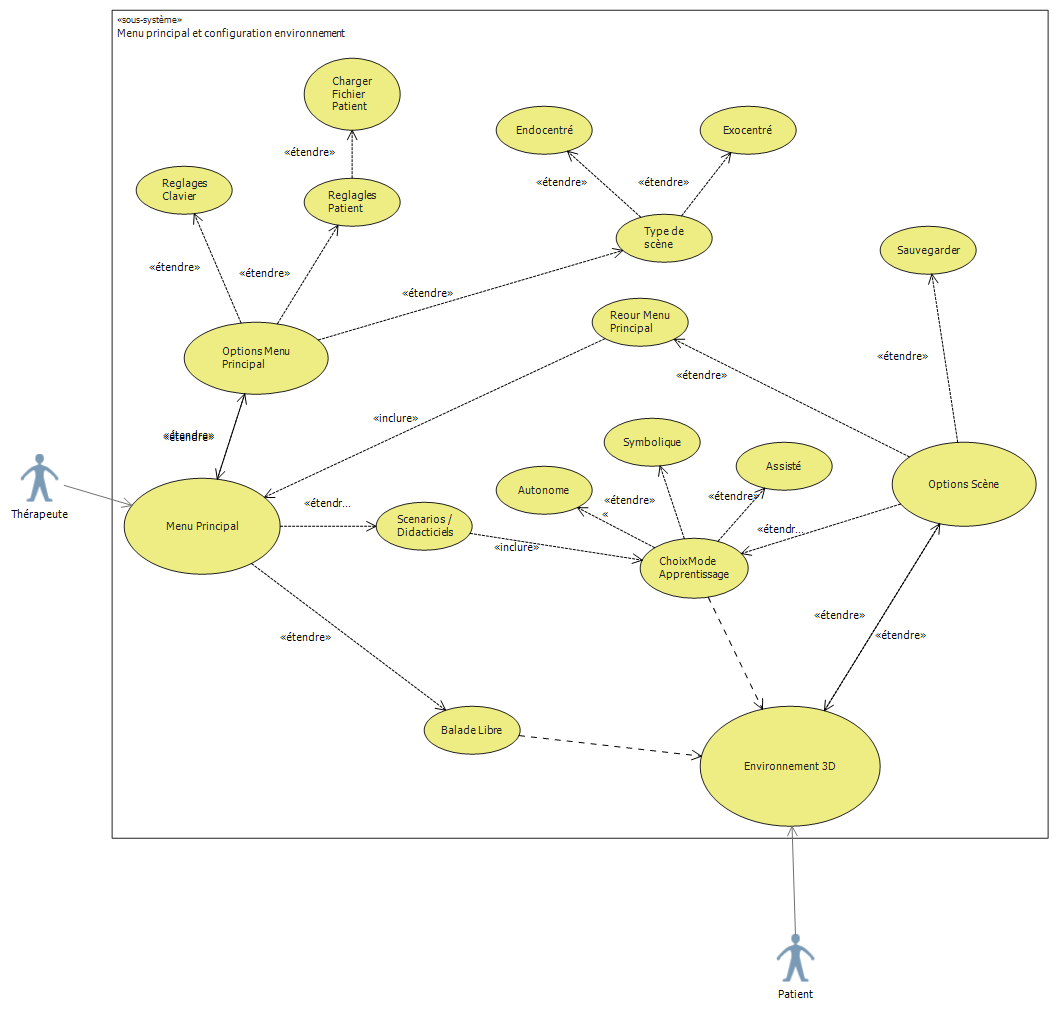
\includegraphics[width=1\textwidth]{2-Specifications/img-utilisateur/cas-usage-menu.png}
\caption{\label{fig:CasUsageMenu} Diagramme de cas d'usage : Menu principal et configurations environnement }
\end{figure}
\FloatBarrier 


\subsubsection{Utilisateur}
Finalement, l'utilisateur n'a accès qu'à la scène. Il peut ainsi interagir avec les objets en fonction du Scénario et du mode d'Apprentissage. Il n'a pas à se soucier des configurations. En parallèle le thérapeute peut vérifier si les actions sont effectués comme prévu et réajuster le mode d'apprentissage ou changer de type de vue si nécessaire.

\pagebreak
\section{Architecture générale}
	\subsection{Briques logicielles}
		Notre projet peut être séparé en plusieurs briques logicielles ; celles-ci correspondent à une première ébauche de l'architecture globale du programme.
		\subsubsection{Moteur de rendu : Unity}
			La première brique est Unity; nous l'utiliserons ici pour sa composante moteur de jeu et environnement de développement, et non pour ses fonctionnalités de création d'objets 3d et ... 
		\subsubsection{Gestion des périphériques : MiddleVR}
			(DEJA FAIT en 2)Raison de son utilisation (multiples périphériques …)
		\subsubsection{Interactions avec les objets}
			Nous allons devoir développer un systême d'interractions entres les objets, pour qu'une action sur un objet ait un effet sur un autre objet.
		\subsubsection{Gestion des scénarios}
			Les scénarios demandés dans le cahier des charges devront être implémentés; il pourrait être appréciable que de nouveaux scénarios puissent facilement être ajoutés.
			De ce fait, nous avons besoin d'un système de gestion des scénarios qui devra par exemple donner l'ordre de différentes actions à réaliser par l'utilisateur, et d'éventuelles aides supplémentaires s'il devait réaliser une action autre que celle demandée.
		\subsubsection{Gestions des objets manipulables}
			Nous devrons aussi implémenter de quoi gérer les objets, pour pouvoir les retrouver et les gérer dans l'espace.
		\subsubsection{Menu}
			Un menu devra être disponible au lancement de l'application, ainsi qu'au cours de l'utilisation.
	\subsection{Liens entre les modules}

%MiddleVR <=> Unity
%Gestionnaire d’objets <=> Objets
%Gestionnaire scénarios <=> Gestionnaire d’objets
\pagebreak
\section{Conclusion}

Nous avons donc choisi une méthode fortement inspirée du cycle de production en V mais en la mêlant à des méthodes agiles pour pouvoir présenter le projet à nos clients régulièrement. Ainsi si chaque jalon du projet, représenté par un livrable à rendre, correspond à une étape de notre cycle en V, nous prévoyons en parallèle d'avancer le développement de l'application, en en présentant les itérations successives à Jean-Paul Departe et Willy Allègre. \newline

Ainsi, nos commanditaires peuvent valider notre avancée en quasi-temps réel. De plus, d'après l'audit réalisé sur Microsoft Project, nous disposons d'une planification correcte. Les différents livrables seront réalisés dans les temps et les estimations que nous avons faites tiennent compte des contre-temps que nous sommes susceptibles de rencontrer et devraient suffire à absorber les retards.
\pagebreak
\bibliography{2-Specifications/biblio}

\end{document}
